\chapter{Project Risk Analysis}
\section{What is risk?}
Risk is a condition where there is a possibility of adverse deviation from a desired and expected outcome. Risk is caused by a lack of precise knowledge regarding future business conditions, technological development, synergies among projects etc. Decisions under risk are decisions in which the analyst models the decision problem in terms of assumed possible future outcomes, or scenarios, whose probabilities of occurrence can be estimated.
\subsection{Sources of uncertainty}
Factors that affect uncertainty in modelling future economic consequences of an engineering project are:
\begin{itemize}
    \item Possible inaccuracy of the cash-flow estimates
    \item The type of business involved in relation to the future health of the economy
    \item The type of physical plant and equipment involved
    \item Length of the study period used
\end{itemize}
\section{Measuring risk}
\subsection{Random variables}
Factors that have probabilistic outcomes (e.g., sots, revenues, useful life) are called random variables. Capital letters $X$, $Y$, $Z$, are usually used to represent random variables and lowercase letters $x$, $y$, $z$ are used to denote the particular values these variables take on in the \textit{sample space}\footnote{Sample space: the set of all possible outcomes for each variable.}. Information about random variables that is particularly helpful for risk analysis is their expected value and variances. Random variables can be defined as either discrete or continuous.
\subsection{Discrete random variables}
A random variable $X$ is said t o be discrete if it can take on at most a countable (finite) number of values ($x_1, x_2, \dots, x_L$). The probability that a discrete random variable $X$ takes on the value $x_i$ is given by:
\begin{equation}
    \textrm{Pr} \left\{X = x_i \right\} = P\left(x_i\right) \textrm{ for } i = 1,2,\dots , L
\end{equation}
where $i$ is the sequential index of the discrete values and $p\left(x_i\right) \geq 0$ and $\sum_i p\left(x_i\right) = 1$.

The probability that the value of $X$ is contained in the closed interval $\left[a,b\right]$ is given by the probability mass function:
\begin{equation}
    \textrm{Pr} \left\{ a \leq X \leq b \right\} = \sum_{ i:a\leq X_i \leq b } p\left(x_i\right)
\end{equation}
The probability that the value of $X$ is less than or equal to $h$ is given by the cumulative distribution function:
\begin{equation}
    \textrm{Pr} \left\{ X \leq h\right\} = p\left(h\right) = \sum_{i:X_i\leq h} p\left(x_i\right)
\end{equation}
In most practical cases, discrete random variables represent countable data such as:
\begin{itemize}
    \item The number of defective columns in a building
    \item The number of maintenance jobs per week
    \item The number of employees
\end{itemize}
\subsection{Continuous random variables}
A random variable $X$ is said to be continuous if it can take on any value within a set of real number $\left[c,d\right]$. The probability that a continuous random variable $X$ takes on a value within the set $\left[c,d\right]$ is given by:
\begin{equation}
    \textrm{Pr}\left\{c\leq X \leq d\right\} = \int_c^d f\left(x\right)\dif x
\end{equation}
where $\int_{\infty}^{\infty}f\left(x\right)\dif x = 1$.

The probability that the value of $X$ assumes exactly any one of its values is 0. The probability that the value of $X$ is less than or equal to $h$ is given by the cumulative distribution function:
\begin{align}
    \textrm{Pr}\left\{X\leq h\right\}         & = F\left(h\right) = \int_{-\infty}^h f\left(x\right)\dif x            \\
    \textrm{Pr}\left\{c \leq X \leq d\right\} & = \int_c^d f\left(x\right) \dif x = F\left(d\right) - F\left(c\right)
\end{align}
In most practical cases, continuous random variables represent measured data such as:
\begin{itemize}
    \item Time
    \item Cost
    \item Revenue
\end{itemize}
\subsection{Expected value}
The expected value of a random variable $X$ is denoted as $E\left(X\right)$. $E\left(X\right)$ is a weighted average of the distribution values of $x$ that it takes on and is a measure of the central location of the distribution. $E\left(X\right)$ is called the mean (or central / first moment) of the distribution.

For a discrete random variable:
\begin{equation}
    E\left(X\right) = \sum_i x_i p\left(x_i\right)
\end{equation}
For a continuous random variable:
\begin{equation}
    E\left(X\right) = \int_{-\infty}^{\infty} x f\left(x\right)\dif x
\end{equation}
\subsection{Variance}
The variance of a random variable $X$ is denoted as $V\left(X\right)$. $V\left(X\right)$ is a measure of the dispersion of the values $X$ takes on around $E\left(X\right)$ (note that the square root of $V\left(X\right)$ is equal to the standard deviation $SD\left(X\right)$). $V\left(X\right)$ is called the second moment of the distribution.

For a discrete random variable:
\begin{equation}
    V\left(X\right) = \sum_i \left[x_i - E\left(X\right)\right]^2 p\left(x_i\right)
\end{equation}
For a continuous random variable:
\begin{equation}
    V\left(X\right) = \int_{-\infty}^{\infty} \left[x - E\left(X\right)\right]^2 f\left(x\right) \dif x
\end{equation}
\subsection{Multiplying by a constant}
Random variables are commonly multiplied by a constant value. e.g.:
\begin{itemize}
    \item The estimated maintenance labour expense for a time period $Y = cX$, where the number of labour hours per period is a random variable $X$ and the cost per labour hour $c$ is constant.
\end{itemize}
For a discrete random variable:
\begin{equation}
    E\left(cX\right) = cE\left(X\right) = c\sum_i x_i p\left(x_i\right)
\end{equation}
For a continuous random variable:
\begin{equation}
    E\left(cX\right) = cE\left(X\right) = c \int_{-\infty}^{\infty} x f\left(x\right) \dif x
\end{equation}
For both random variable types:
\begin{equation}
    V\left(cX\right) = c^2 V\left(X\right)
\end{equation}
\subsection{Multiplying by another random variable}
Sometimes a random variable $Z$ results from the product of two other independent random variable $(XY)$, e.g.:
\begin{itemize}
    \item The estimated annual expenses $Z$ for a repair part repetitively procured during the year on a competitive basis, when the unit price $X$ and the number of units used per year $Y$ are independent random variables.
\end{itemize}
The expected value of $Z$ is:
\begin{equation}
    E\left(Z\right) = E\left(X\right)E\left(Y\right)
\end{equation}
The variance of $Z$ is:
\begin{equation}
    V\left(Z\right) = E\left[XY - E\left(XY\right)\right]^2 = E\left(X^2\right)E\left(Y^2\right)- \left[E\left(X\right)E\left(Y\right)\right]^2
\end{equation}
\subsection{Adding or subtracting random variables}
Sometimes a random variable (Z) results from adding or subtracting two independent variables ($X+Y$ or $X-Y$) e.g.:
\begin{itemize}
    \item Alternative A has a cost of $X$ and alternative B has a cost of $Y$. The probability that alternative A is less costly than alternative B is equal to:
          \begin{equation}
              \textrm{Pr}\left\{X < Y \right\} = \textrm{Pr}\left\{ X-Y < 0\right\} = \textrm{Pr} \left\{ Z < 0\right\}
          \end{equation}
\end{itemize}
The expected value of $Z$ is:
\begin{equation}
    E\left(Z\right) = E\left(X\right) \pm E\left(Y\right)
\end{equation}
The variance of $Z$ is:
\begin{equation}
    V\left(Z\right) = V\left(X\right) + V\left(Y\right)
\end{equation}
\section{Example risk analysis}
\subsection{Worked example 1}
Suppose that the estimated probability of obtaining various capacity utilisations in a premixed-concrete plant project are as follows:
\begin{table}[H]
    \centering
    \begin{tabular}{@{}llll@{}}
        \toprule
        \textbf{Capacity (\%)} & \textbf{Probability} & \textbf{Annual Revenue} & \textbf{AV (15\%)} \\
        \midrule
        50                     & 0.10                 & \pounds 405,000         & -\pounds 25,093    \\
        65                     & 0.30                 & \pounds 526,500         & \pounds 22,136     \\
        75                     & 0.50                 & \pounds 607,500         & \pounds 53,622     \\
        90                     & 0.10                 & \pounds 729,000         & \pounds 100,850    \\
        \bottomrule
    \end{tabular}
    \caption{Worked example 1 table.}
\end{table}
\begin{quoting}
    Estimate $E\left(AV\right)$ and $V\left(AV\right)$
\end{quoting}
\begin{gather}
    E\left(X\right) = \sum_i x_i p\left(x_i\right)\\
    E\left(AV\right) = 0.1 \times -25903 + 0.3 \times 22136 + 0.5 \times 53622 + 0.1 \times 100850 = \pounds 41,028\\
    V\left(X\right) = \sum_i \left[x_i - E\left(X\right)\right]^2 p\left(x_i\right)
\end{gather}
\begin{multline}
    V\left(AV\right) = 0.1 \times \left(-25903 - 41028\right)^2 + 0.3 \times \left(22136 - 41028\right)^2 + \\
    0.5 \times \left(53622 - 41028\right)^2 + 0.1 \times \left(100850 - 41028\right)^2 = \pounds\SI{9.9e8}{}
\end{multline}
\begin{align}
    E\left(AV\right)        & = \pounds 41,028       \\
    V\left(AV\right)        & = \pounds \SI{9.9e8}{} \\
    \sqrt{V\left(AV\right)} & = \pounds 31,327
\end{align}
By evaluating both $E\left(AV\right)$ and $V\left(AV\right)$ for the concrete plant, indications of the venture's average profitability and riskiness are obtained. The mean value is above one standard deviation from \pounds 0. This leads to the conclusion that there is low risk, and that this is a good investment.
\subsection{Risk analysis with continuous random variables}
Supposed that the NPV of a project is \pounds 153 and the corresponding variance is \pounds 484,416. If the NPV is a normally distributed\footnote{Commonly used distribution that is easy to calculate using a computer and can be entirely described by the mean and variance parameters.} random variable, what is the probability of having a negative NPV?

From Excel, use \texttt{=norm.dist(0,E(NPV),sqrt(V(NPV)),1)}. The first value is 0, because we want to find the probability of it being less than the mean. The last 1 gives us the cumulative distribution. This results in a 41.3\% of having a NPV less than 0.
\begin{equation}
    \textrm{Pr}\left\{ NPV \leq 0\right\} = F(0) = \int_{-\infty}^0 f\left(npv\right)\dif npv = 0.413
\end{equation}
\subsection{Risk analysis with multiple independent random variables}
Suppose that the estimated cash flow data for a project are show in the following table for a five-year study period. Each annual net cash-flow amount, $F_k$, is a linear combination of two statistically independent random variables, $X_k$ and $Y_k$, where $X_k$ is a revenue factor and $Y_k$ is an expense factor. The $X_k$ cash-flow amounts are statistically independent of each other, and the same is true of the $Y_k$ amounts. Both $X_k$ and $Y_k$ are continuous random variables, but the form of their probability distributions is not known. Interest rate is 20\% per year.
\begin{quoting}
    Estimate $E\left(NPV\right)$, $V\left(NPV\right)$ and $SD\left(NPV\right)$ of the project's cash flows.
\end{quoting}
\begin{table}[H]
    \centering
    \begin{tabular}{@{}llllll@{}}
        \toprule
        \textbf{End of year} $k$ & \textbf{Net cash flow} & $E\left[X_k\right]$ & $E\left[Y_k\right]$ & $SD\left[X_k\right]$ & $SD\left[Y_k\right]$ \\
        \midrule
        0                        & $F_0 = X_0 + Y_0$      & \pounds 0           & -\pounds 100,000    & \pounds 0            & \pounds 10,000       \\
        1                        & $F_1 = X_1 + Y_1$      & \pounds 60,000      & -\pounds 20,000     & \pounds 4,500        & \pounds 2,000        \\
        2                        & $F_2 = X_2 + 2Y_2$     & \pounds 65,000      & -\pounds 15,000     & \pounds 8,000        & \pounds 1,200        \\
        3                        & $F_3 = 2X_3 + 3Y_3$    & \pounds 40,000      & -\pounds 9,000      & \pounds 3,000        & \pounds 1,000        \\
        4                        & $F_4 = X_4 + 2Y_4$     & \pounds 70,000      & -\pounds 20,000     & \pounds 4,000        & \pounds 2,000        \\
        5                        & $F_5 = 2X_5 + 2Y_5$    & \pounds 55,000      & -\pounds 18,000     & \pounds 4,000        & \pounds 2,300        \\
        \bottomrule
    \end{tabular}
    \caption{Risk analysis with multiple independent random variables table.}
\end{table}
\begin{align}
    E\left(F_k\right) & = E\left(a_k X_k + b_k Y_k\right) = E\left(a_k X_k\right) + E\left(b_k Y_k\right) = a_k E\left(X_k\right) + b_k E\left(Y_k\right)     \\
    V\left(F_k\right) & = V\left(a_k X_k + b_k Y_k\right) = V\left(a_k X_k\right) + V\left(b_k Y_k\right) = a_k^2 V\left(X_k\right) + b_k^2 V\left(Y_k\right)
\end{align}
\begin{table}[H]
    \centering
    \begin{tabular}{@{}llllllll@{}}
        \toprule
        \textbf{End of year} $k$ & \textbf{Net cash flow} & $E\left[X_k\right]$ & $E\left[Y_k\right]$ & $SD\left[X_k\right]$ & $SD\left[Y_k\right]$ & $E\left[F_k\right]$ & $V\left[V_k\right]$ \\
        \midrule
        0                        & $F_0 = X_0 + Y_0$      & \pounds 0           & -\pounds 100,000    & \pounds 0            & \pounds 10,000       & -\pounds 100,000    & \SI{100e6}{}        \\
        1                        & $F_1 = X_1 + Y_1$      & \pounds 60,000      & -\pounds 20,000     & \pounds 4,500        & \pounds 2,000        & \pounds 40,000      & \SI{24.2e6}{}       \\
        2                        & $F_2 = X_2 + 2Y_2$     & \pounds 65,000      & -\pounds 15,000     & \pounds 8,000        & \pounds 1,200        & \pounds 35,000      & \SI{69.8e6}{}       \\
        3                        & $F_3 = 2X_3 + 3Y_3$    & \pounds 40,000      & -\pounds 9,000      & \pounds 3,000        & \pounds 1,000        & \pounds 53,000      & \SI{45e6}{}         \\
        4                        & $F_4 = X_4 + 2Y_4$     & \pounds 70,000      & -\pounds 20,000     & \pounds 4,000        & \pounds 2,000        & \pounds 30,000      & \SI{32e6}{}         \\
        5                        & $F_5 = 2X_5 + 2Y_5$    & \pounds 55,000      & -\pounds 18,000     & \pounds 4,000        & \pounds 2,300        & \pounds 74,000      & \SI{85.2e6}{}       \\
        \bottomrule
    \end{tabular}
    \caption{Risk analysis with multiple independent random variables table with expected and variance values.}
\end{table}
\begin{align}
    E\left(NPV\right)  & = \sum_{k=0}^5 \dfrac{E\left(F_k\right)}{\left(1+i\right)^n} = \pounds 32,517             \\
    V\left(NPV\right)  & = \sum_{k=0}^5 \dfrac{V\left(F_k\right)}{\left(1+i\right)^{2n}} = \pounds \SI{186.75e6}{} \\
    SD\left(NPV\right) & = \sqrt{V\left(NPV\right)} = \pounds 13,666
\end{align}
\section{Decision trees}
Decision trees are powerful means of depicting and facilitating the analysis of important problems. Decision tress break down a large, complicated problem into a series of smaller, simple problems. They enable objective analysis and decision making that includes explicit consideration of the risk and effect of the future.
\begin{figure}[H]
    \centering
    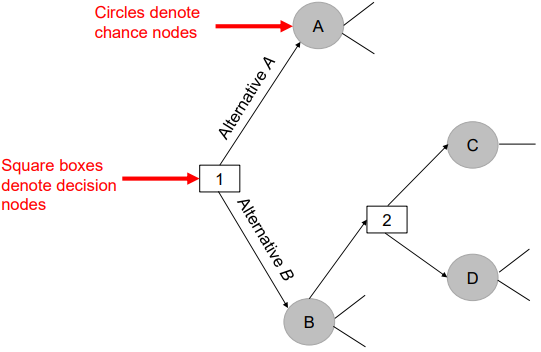
\includegraphics[width = 0.7 \textwidth]{img/figure63.png}
    \caption{Decision tree.}
\end{figure}
\subsection{Worked example of a decision tree}
CEGE Corporation manufactures compressors for commercial air-condition systems. A new compressor design is being evaluated as potential replacement for the most frequently used unit. The new design involves major changes that have the expected advantage of better operating efficiency. From the perspective of a typical user, the new compressor (as an assembled component in an air-conditioning system) would have an increased investment of \pounds 8,600 relative to the present unit and an annual expense saving dependent on the extent to which the design goal is met in actual operation. Estimates by the multidisciplinary design team of the new compressor achieving four levels (percentages) of the efficiency design goal and the probability and annual expense saving at each level are as follows.
\begin{table}[H]
    \centering
    \begin{tabular}{@{}lll@{}}
        \toprule
        \textbf{Level of design goal met (\%)} & \textbf{Probability} $p\left(L\right)$ & \textbf{Annual expense saving} \\
        \midrule
        90                                     & 0.25                                   & \pounds 3,470                  \\
        70                                     & 0.40                                   & \pounds 2,920                  \\
        50                                     & 0.25                                   & \pounds 2,310                  \\
        30                                     & 0.10                                   & \pounds 1,560                  \\
        \bottomrule
    \end{tabular}
    \caption{Decision tree example table.}
\end{table}
\begin{quoting}
    Use MARR = 18\%, an analysis period of 6 years, and $E\left(NPV\right)$ as the decision criterion, is the new compressor design economically preferable to the current unit?
\end{quoting}
Convert to present value figures using the formula for AV.
\begin{figure}[H]
    \centering
    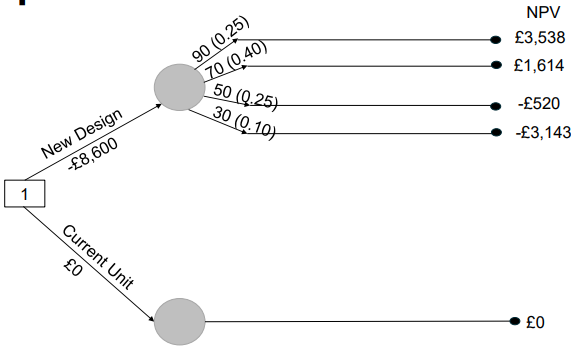
\includegraphics[width = 0.5\textwidth]{img/figure64.png}
    \caption{Decision tree for worked example.}
\end{figure}
\begin{gather}
    E\left(X\right) = \sum_i x_i p\left(x\right)\\
    E\left(NPV\right) = 0.25 \times 3538 + 0.40 \times 1614 + 0.25\times (-520) + 0.10 \times (-3413) = 1086
\end{gather}
There is a 35\% chance of a negative NPV value, hence depending on the risk appetite of the company, we find that this may not be a good investment. However, we do have a positive $E\left(NPV\right)$ value.